We tested our GLM predictions on silver (XAG) commodity pricing data. Our date range of 20130401-20150208 containing 652 days was split into a training set containing 526 days, a validation set containing 59 days, and a test set containing 67 days.\\

For baseline values, we simply take the minimum error for predicting either 0 or 1 (price up or price down) for all days. Our baseline error is 0.48.\\

We trained 54 logistic regression models, varying the number of clusters trained on, the inverse regularization strength $c$, and the type of regularization (L1 or L2). The number of clusters $K$ ranged took values in the set $\{10,20,30,40,50,100,200,300,400,500,1000,2000,3000,4000,5000\}$. $c$ was varied between 0.01−0.1 (stepping by 0.01), 0.1−1 (stepping by 0.1), and 1−10 (stepping by 1).\\

We also tested precision, recall, and f1 scores for various prediction probability cutoffs between 0.1 and 0.9.

The model with the least error was trained on $K$=40, $c$=4, and used L1 regularization and had an error of 0.373. We plot precision vs recall at various cutoffs. 

\begin{figure}[ht]
\vskip 0.2in
\begin{center}
\centerline{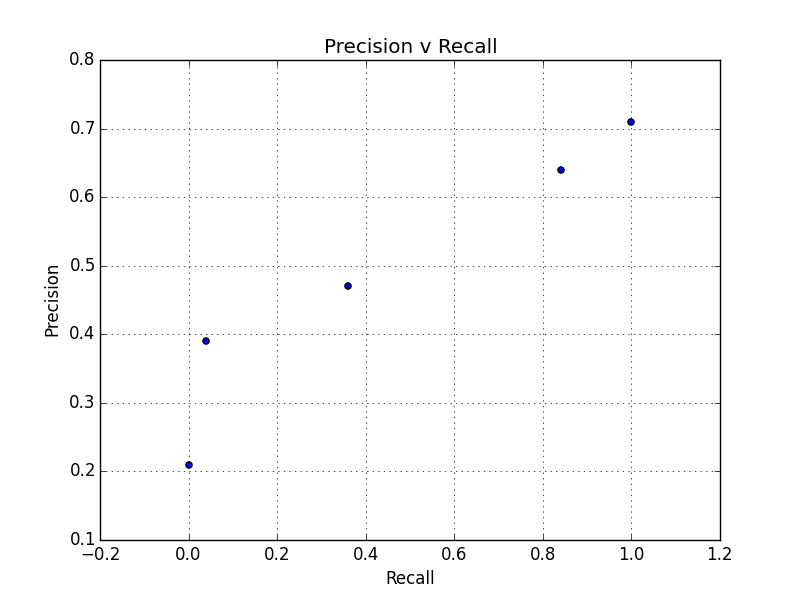
\includegraphics[scale=0.15]{images/precision_v_recall.png}}
\caption{Precision vs Recall for the best model}
\end{center}
\vskip -0.2in
\label{fig:precision_v_recall}
\end{figure} 

Train and test errors as a function of $K$ are shown. Models were retrained 20 times each, with randomized initalization constants. Overall, errors were between 0.4 and 0.6 and seemed to hover around expected baseline errors. 


\begin{figure}[ht]
\vskip 0.2in
\begin{center}
\centerline{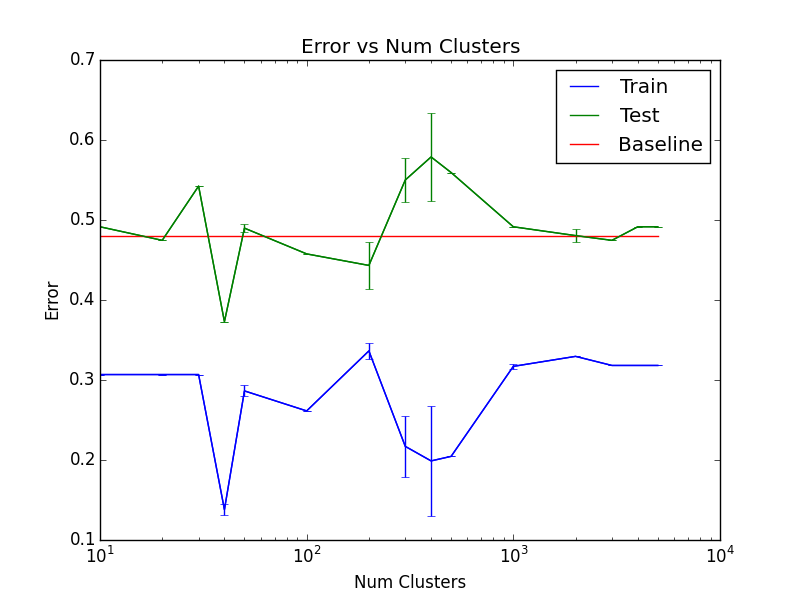
\includegraphics[scale=0.15]{images/error_v_k.png}}
\caption{Error vs Number of Clusters}
\end{center}
\vskip -0.2in
\label{fig:error_v_k}
\end{figure} 

We computed the clusters on the a large part of dataset, but due to time constraints had to run initial predictions on the subset of the data that was clustered and coalesced, which did not at the time include the few most recent months reserved for testing. As a result, test data was used for computing K-means. We think this may inflate test accuracy slightly. However, the clusters were also computed from samples of days far in the future of the test data, so those likely had a cancelling adverse effect. In any case, these initial exploratory results are just hints at a possible signal.
